
\documentclass{article}
\usepackage{tikz}
\begin{document}
    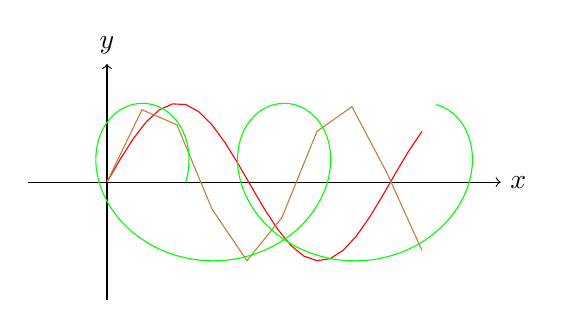
\begin{tikzpicture}
        \draw [->] (-1, 0) -- (5, 0);
        \node at (5, 0) [right] {$x$};
        \draw [->] (0, -1.5) -- (0, 1.5);
        \node at (0, 1.5) [above] {$y$};
        \draw [red] plot [domain=0:4] ({\x}, {sin(100*\x)});
        \draw [brown] plot [domain=0:4, samples=10] ({\x}, {sin(150*\x)});
        \draw [green] plot [domain=0:4, samples=1000]
            ({\x + cos(200*\x)}, {sin(200*\x)});
    \end{tikzpicture}
\end{document}

